\chapter{Задание 1. Вещественное}
\label{ch:chap2}

\definecolor{codegreen}{rgb}{0,0.6,0}
\definecolor{codegray}{rgb}{0.5,0.5,0.5}
\definecolor{codepurple}{rgb}{0.58,0,0.82}
\definecolor{backcolour}{rgb}{0.95,0.95,0.92}

\lstdefinestyle{mystyle}{
    backgroundcolor=\color{backcolour},   
    commentstyle=\color{codegreen},
    keywordstyle=\color{magenta},
    numberstyle=\tiny\color{codegray},
    stringstyle=\color{codepurple},
    basicstyle=\ttfamily\footnotesize,
    breakatwhitespace=false,         
    breaklines=true,                 
    captionpos=b,                    
    keepspaces=true,                 
    numbers=left,                    
    numbersep=5pt,                  
    showspaces=false,                
    showstringspaces=false,
    showtabs=false,                  
    tabsize=2
}
\lstset{style=mystyle}


\textit{NB.} - В этом задании мы используем унитарное преобразование Фурье к угловой частоте $\omega$, оно будет выглядеть следующим образом: 

\begin{itemize}
    \item Исходная функция
    $$
    f(t) = \frac{1}{\sqrt{2\pi}}\int^{+\infty}_{-\infty}c(\omega)e^{i\omega t}d\omega
    $$
    \item Фурье-образ
    $$
    c(\omega) = \frac{1}{\sqrt{2\pi}}\int^{+\infty}_{-\infty}f(t)e^{-i\omega t}dt
    $$

  \end{itemize}

Теперь рассмотрим следующие функции $f: \mathbb{R} \rightarrow \mathbb{R}$

\section{Прямоугольная функция}
$$
f(t) = \begin{cases}
    a, |t| \leq b, \\
    0, |t|>b
\end{cases}
$$

\subsection{Фурье-Образ}
$\hat{f_1}(\omega) = \frac{1}{\sqrt{2\pi}}\int^{+\infty}_{-\infty}(\dots)dt = \frac{1}{\sqrt{2\pi}}\bigg[\int^{-b}_{-\infty}0 dt + \int^{b}_{-b}ae^{-i\omega t}dt + \int^{+\infty}_{b}0 dt \bigg]=
\frac{a}{\sqrt{2\pi}}\int^{b}_{-b}e^{-i\omega t}dt = \frac{a}{-i\omega \sqrt{2\pi}}e^{-i\omega t}\Bigr|_{-b}^{b} = \frac{2a}{-2i\omega \sqrt{2\pi}}(e^{-i\omega b} - e^{i\omega b}) = \frac{2ab}{2ib\omega \sqrt{2\pi}}(e^{i\omega b} - e^{-i\omega b}) = 
\frac{2ab}{b\omega \sqrt{2\pi}}sin(\omega b) = \frac{2ab}{\sqrt{2\pi}}\cdot sinc(\omega b)$

\subsection{Графики функции и Фурье-образа}


\begin{figure}[ht]
    \centering
    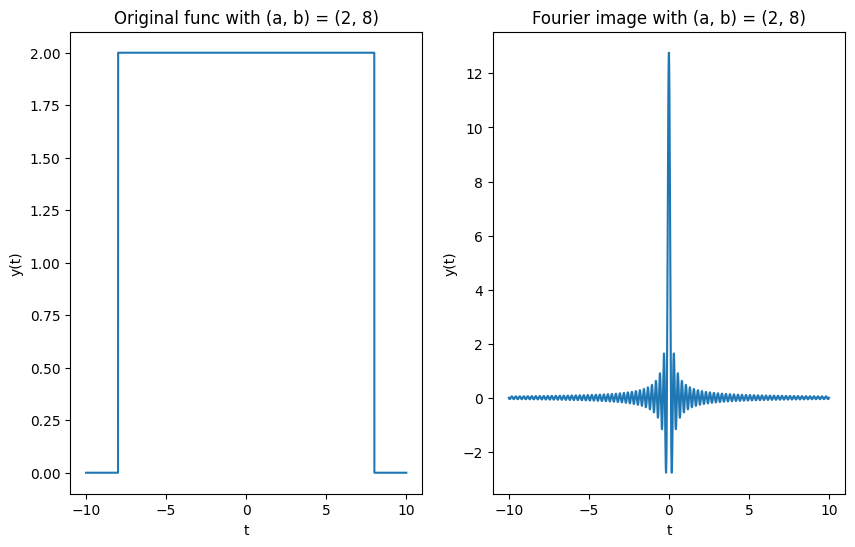
\includegraphics[width=0.9\textwidth]{f1_1.png}
    \caption{График и образ прямоугольной функции}
\end{figure}

\begin{figure}[ht]
    \centering
    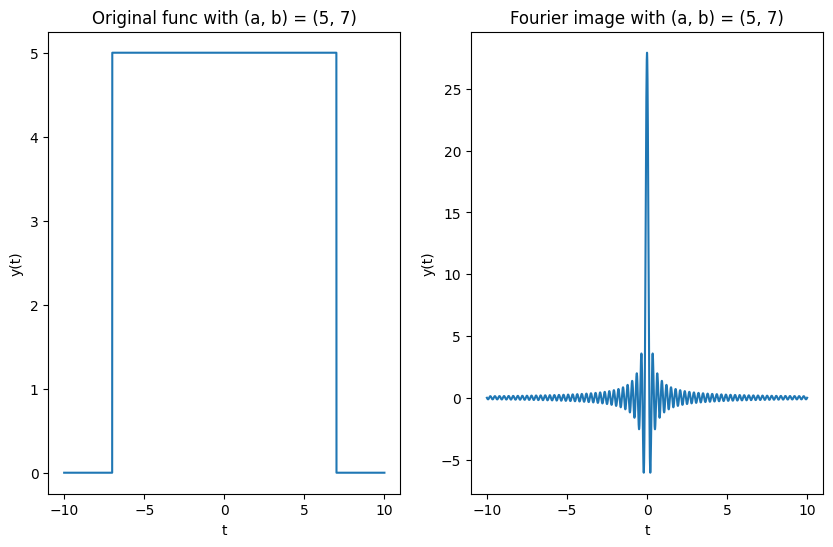
\includegraphics[width=0.9\textwidth]{f1_2.png}
    \caption{График и образ прямоугольной функции}
\end{figure}

\begin{figure}[ht]
    \centering
    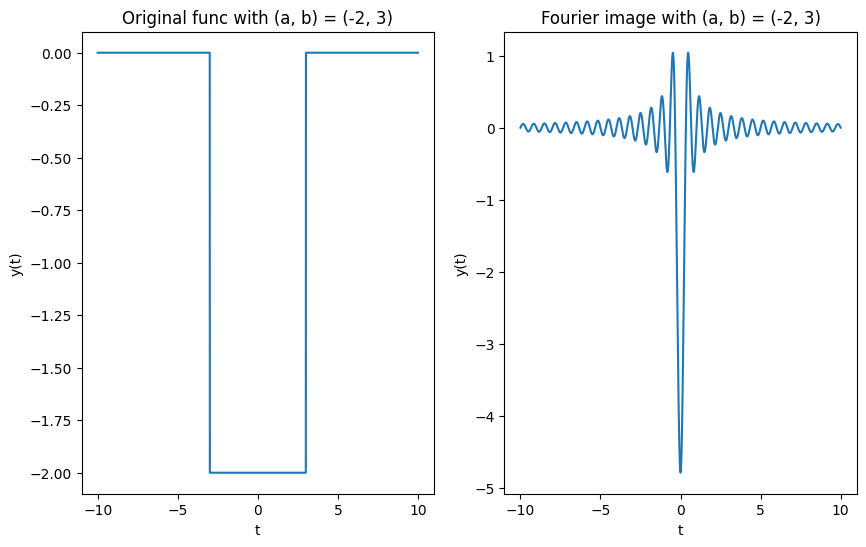
\includegraphics[width=0.9\textwidth]{f1_3.png}
    \caption{График и образ прямоугольной функции}
\end{figure}

\begin{figure}[ht]
    \centering
    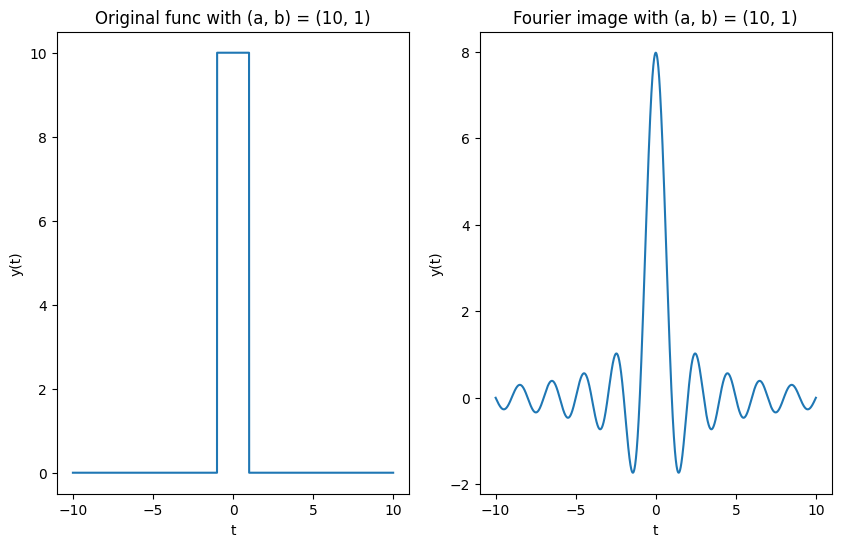
\includegraphics[width=0.9\textwidth]{f1_4.png}
    \caption{График и образ прямоугольной функции}
\end{figure}
\newpage
\subsection{Равенство Парсеваля}

Проверим равенство Парсеваля, в нашем случае оно будет выглядеть следующим образом
$$
||f||_2 = ||\mathbb{F}f||_2
$$, где $\mathbb{F}$ - оператор Фурье, а норму вектора определим как корень из суммы квадратов всех его компонент.

Также вспомним про то, что применение оператора Фурье на функцию равняется её фурье образу, поэтому
$$
\mathbb{F}f = \hat{f}
$$ А значит можно записать равенство Парсеваля в более приближенной форме для численных приближений
\begin{align*}
    \int_{-\infty}^{+\infty}|f(t)|^2dt = \int_{-\infty}^{+\infty}|\hat{f}(\omega)|^2dt \\
    \bigg(  \int_{-\infty}^{+\infty}|f(t)|^2dt - \int_{-\infty}^{+\infty}|\hat{f}(\omega)|^2dt \bigg) \rightarrow 0
\end{align*}
Удобно отслеживать не равенство левой и правой части, а стремление их разности к нулю, так и поступим.

Полезно также знать, что оно имеет физическое значение: \textit{равенство энергии сигнала во временной области и энергетического спектра в частотной области}.
Правда, так как я не физик, то чёткого значения этих слов я не понимаю...

Второе полезное замечание: по неизвестной мне причине, привычное scipy интегрирование не очень хорошо работало на первую функцию, возможно из-за её бесконечной переодичности интеграл расходился,
но когда вместо границ [-np.inf ; +np.inf] я поставил просто большие числа, например, $[-10^7 ; 10^7]$, то результаты уже стали человечнее...

Получил в нашем случае \texttt{delta: 0.01363}, подробности вычислений смотрите в используемых функциях или в онлайн-блокноте

\subsection{Анализ ситуации}

В данном случае заметная следующая тенденция - при увеличении ширины волны, частота Фурье образа взрастает, он становится "сжатым"...

Принцип неопределённости можно привязать здесь следующим образом - чем более концентрированной является функция $f(t)$, тем более разнесенным должно быть её  преобразование Фурье $\hat{f}(\omega)$. В частности, такое свойство можно рассматривать как утверждение: если мы сжимаем функцию в t раз, то её преобразование Фурье растягивается на $\omega$.
\textbf{Невозможно} произвольно сконцентрировать как функцию, так и её преобразование Фурье.

Спасибо за это силе википедии, \href{https://en.wikipedia.org/wiki/Uncertainty_principle?useskin=vector}{Принцип неопределённости}, \href{https://en.wikipedia.org/wiki/Fourier_transform?useskin=vector}{Преобразование Фурье}

\section{Треугольная функция}
$$
f(t) = \begin{cases}
    a-|at/b|, |t| \leq b, \\
    0, |t|>b
\end{cases}
$$


\subsection{Фурье-Образ}

Внутри нам встрется до жути уже знакомые интегралы или интегрирование по частям, поэтому я их пропускал, чтобы слишком подробно не расписывать, также воспользуемся старым приёмом: 
разделяем на два интеграла, раскрывая модуль, решаем каждый по отдельности:

$\hat{f_2}(\omega) = \frac{1}{\sqrt{2\pi}}\int^{+\infty}_{-\infty}(a-|at/b|)\cdot e^{-i\omega t} dt =  \frac{1}{\sqrt{2\pi}}\bigg[\int^{-b}_{-\infty}0 dt + \int^{0}_{-b}(a + \frac{at}{b})e^{-i\omega t}dt + \\ \int^{b}_{0}(a - \frac{at}{b})e^{-i\omega t}dt + \int^{+\infty}_{b}0dt \bigg]=$ \\
Воспользуемся линейностью интегралов и перегруппируем слагаемые:
$\frac{1}{\sqrt{2\pi}}\bigg( \frac{a(ib\omega - e^{ib\omega} + 1)}{b\omega^2} + \frac{a(-ib\omega - e^{-ib\omega} + 1)}{b\omega^2} \bigg) = \frac{1}{\sqrt{2\pi}}\bigg( \frac{a(- e^{-ib\omega} - e^{ib\omega} + 2)}{b\omega^2}  \bigg) = \frac{1}{\sqrt{2\pi}}\bigg( \frac{4a\sin^2(b\omega/2)}{b\omega^2}  \bigg) = \frac{4a\sin^2(b\omega/2)}{\sqrt{2\pi} b\omega^2} = \frac{ab}{\sqrt{2\pi}}sinc^2(\frac{b\omega}{2})$

\newpage
\subsection{Графики функции и Фурье-образа}

\begin{figure}[ht]
    \centering
    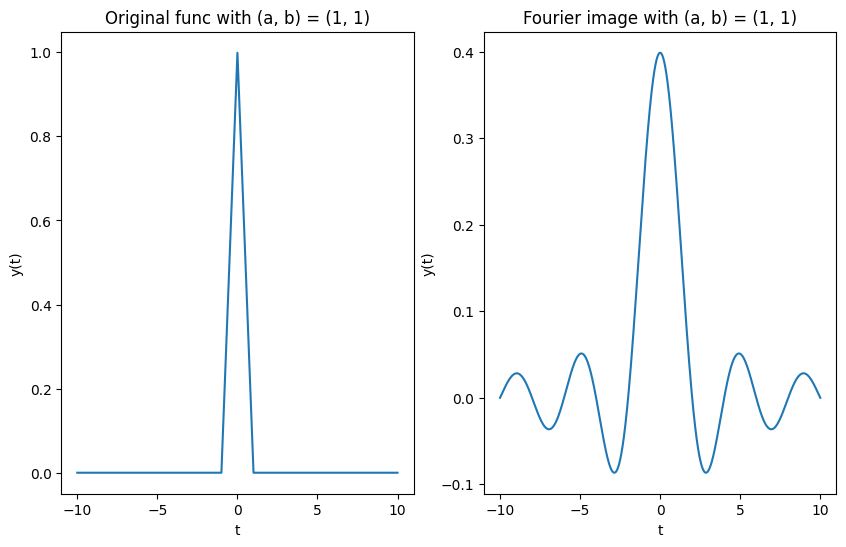
\includegraphics[width=0.9\textwidth]{f2_1.png}
    \caption{График и образ треугольной функции}
\end{figure}

\begin{figure}[ht]
    \centering
    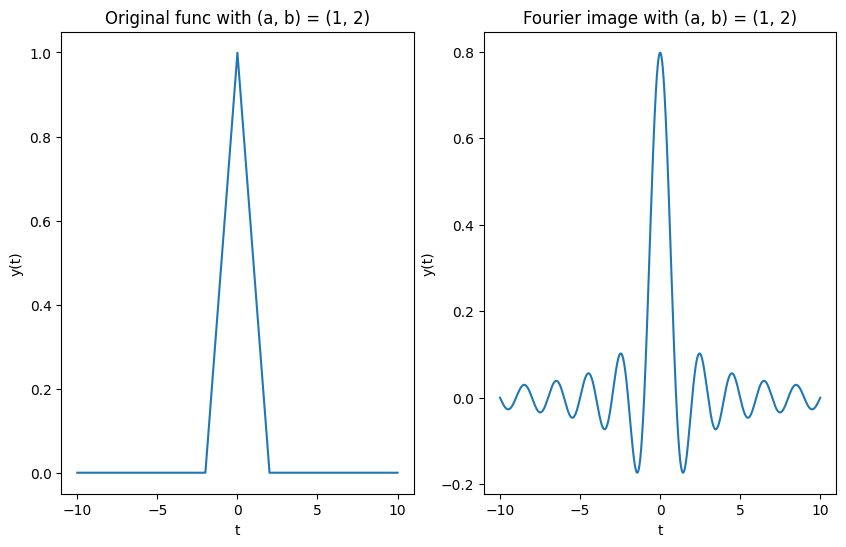
\includegraphics[width=0.9\textwidth]{f2_2.png}
    \caption{График и образ треугольной функции}
\end{figure}

\begin{figure}[ht]
    \centering
    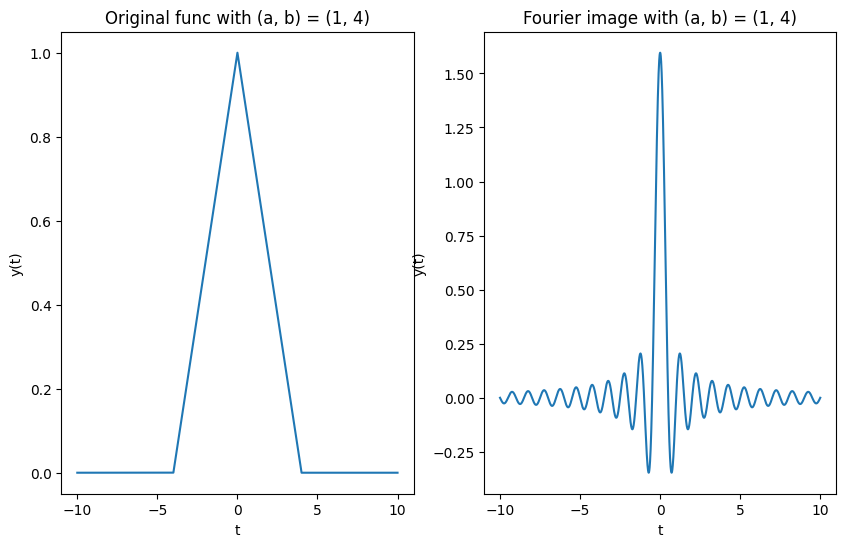
\includegraphics[width=0.9\textwidth]{f2_3.png}
    \caption{График и образ треугольной функции}
\end{figure}

\begin{figure}[ht]
    \centering
    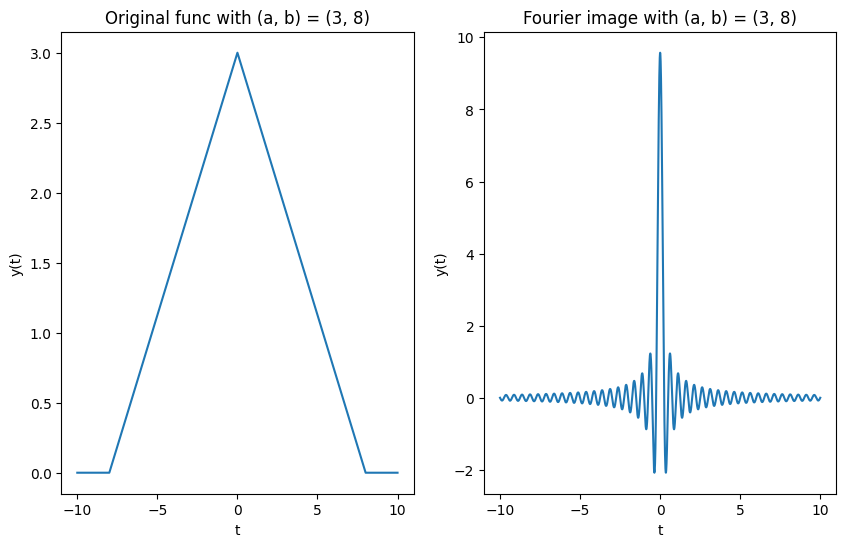
\includegraphics[width=0.9\textwidth]{f2_4.png}
    \caption{График и образ треугольной функции}
\end{figure}
\newpage

\subsection{Равенство Парсеваля}

Получил \texttt{delta: 0.22765}

\subsection{Анализ ситуации}

Влияние параметров $a$ и $b$ на исходную функцию и образ можно увидеть из того, как они заданы. Параметр $a$ определяет высоту
треугольной функции, $a$ параметр $и$ — "ширину основания". В образе функции видно, что
при увеличении параметра $a$ амплитуда образа увеличивается, а при увеличении параметров
$a$ и $b$ амплитуда увеличивается, при увеличении параметра $b$ увеличивается частота.

Принцип неопределенности, как и в прошлом случае, можно увидеть как уменьшение
ширины образа при увеличении основания треугольника.

\section{Кардинальный синус}
$$
f(t) = asinc(bt)
$$


\subsection{Фурье-Образ}
Из-за свойств оператора Фурье нетрудно понять, что Фурье-образ будет прямоугольник из первого пункта, но нужно точно понимать в каком виде он там будет представлен.
Для этого всё же интеграл придётся взять, но без силы интернета я не смог справится, \href{https://math.stackexchange.com/questions/736749/fourier-transform-of-sinc-function}{например}, этот источник предлагает свести его к двойному и с помощью теоремы Фубини разрулить ситуацию...поверим ему и воспользуемся готовеньким:


$$\hat{f_3}(\omega) = \frac{a\pi}{2\sqrt{2\pi}}[ sign(\omega + b) - sign(\omega - b) ]$$

\subsection{Графики функции и Фурье-образа}

\begin{figure}[ht]
    \centering
    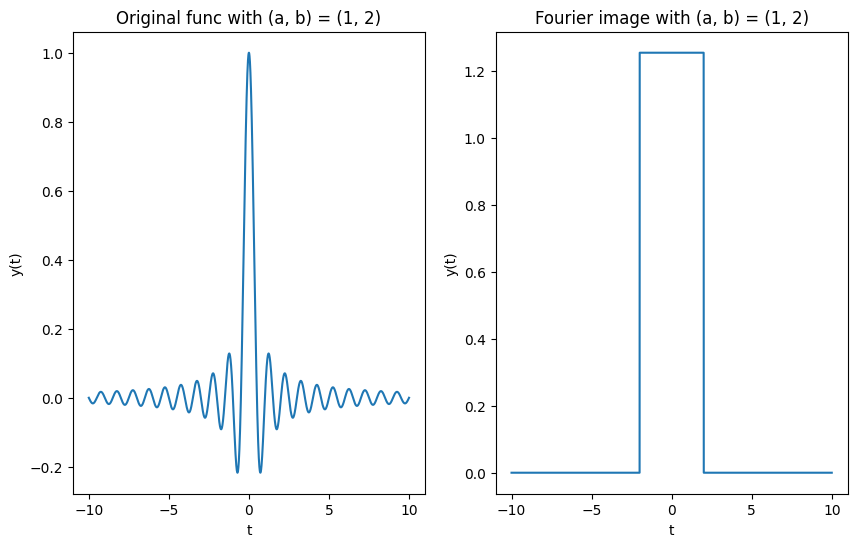
\includegraphics[width=0.9\textwidth]{f3_1.png}
    \caption{График и образ кардинального синуса}
\end{figure}

\begin{figure}[ht]
    \centering
    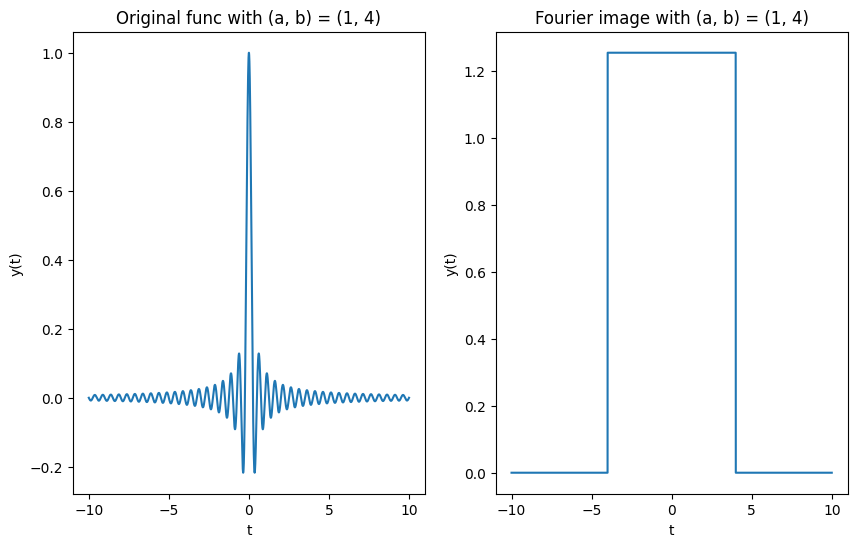
\includegraphics[width=0.9\textwidth]{f3_2.png}
    \caption{График и образ кардинального синуса}
\end{figure}

\begin{figure}[ht]
    \centering
    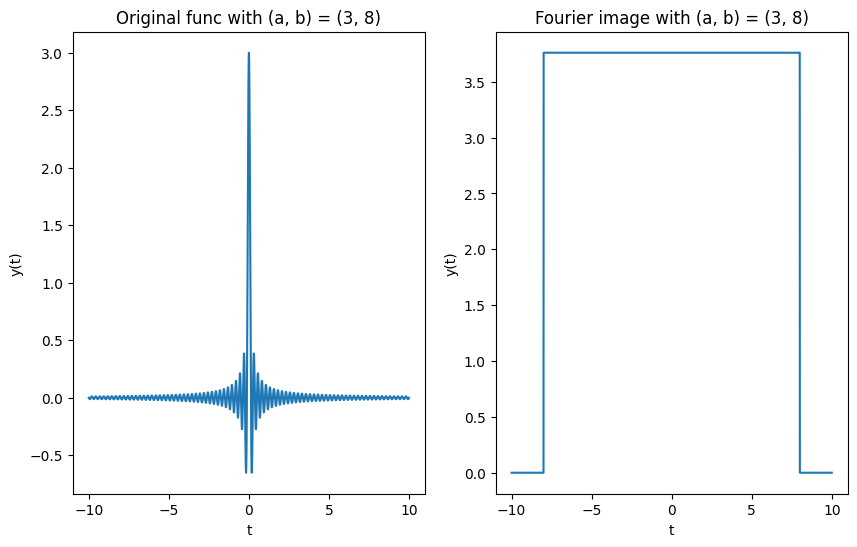
\includegraphics[width=0.9\textwidth]{f3_3.png}
    \caption{График и образ кардинального синуса}
\end{figure}

\subsection{Равенство Парсеваля}

Получил \texttt{delta: 0.01842}, что довольно неплохое приближение, учитывая, что равенство выполняется лишь на бесконечности


\subsection{Анализ ситуации}
Получается, что параметр $a$ отвечает за длину прямоугольника изображения, 
а значит и главный горбик функции, параметр $b$ - за растяжение/сжатие прямоугольника, 
и следовательно, за сжатие/растяжение исходной функции...

Принцип неопределенности проявляется ровно также, как и в первой функции: 
при уменьшении ширины кардинального синуса увеличивается ширина его
образа.

\section{Функция Гаусса}
$$
f(t) = ae^{-bt^2}
$$


\subsection{Фурье-Образ}
Воспользуемся известным фактом из \href{https://ru.wikipedia.org/wiki/%D0%93%D0%B0%D1%83%D1%81%D1%81%D0%BE%D0%B2_%D0%B8%D0%BD%D1%82%D0%B5%D0%B3%D1%80%D0%B0%D0%BB?useskin=vector}{википедии} об Гауссовом интеграле:
$$
\int_{-\infty}^{+\infty}e^{-(Ax^2+Bx+C)}dx = \sqrt{\frac{\pi}{A}}e^{\frac{B^2}{4A}-C}
$$
Тогда вычисления значительно упростятся...
$$\hat{f_4}(\omega) = \frac{a}{\sqrt{2\pi}}\int_{-\infty}^{+\infty}e^{-bt^2}e^{-i\omega t} = \frac{a}{\sqrt{2\pi}}\int_{-\infty}^{+\infty}e^{-(bt^2 + i\omega t)}dx$$
, где $A=b$, $B=i\omega$, $C=0$, тогда\dots
$$
\hat{f_4}(\omega) = a\sqrt{\frac{\pi}{2\pi b}}e^{\frac{(i\omega)^2}{4b}} = \frac{a}{\sqrt{2b}}e^{-\frac{\omega^2}{4b}}
$$

\newpage
\subsection{Графики функции и Фурье-образа}

\begin{figure}[ht]
    \centering
    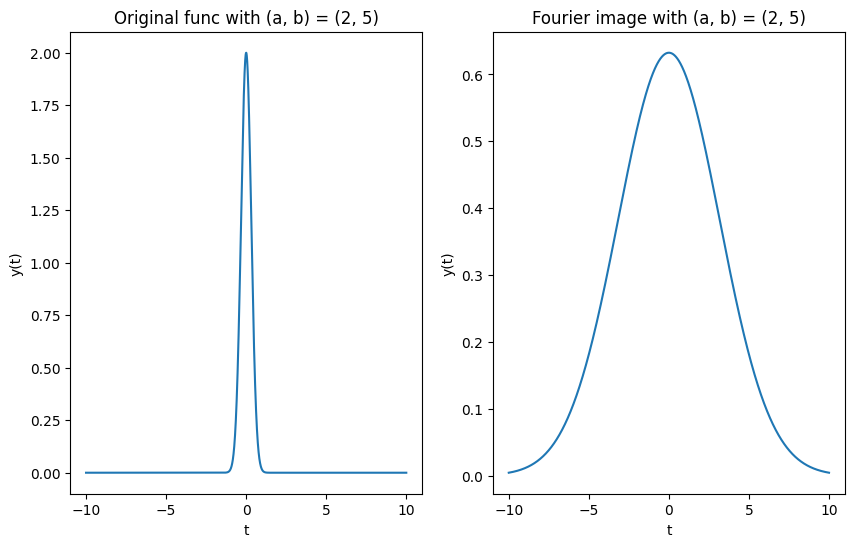
\includegraphics[width=0.9\textwidth]{f4_1.png}
    \caption{График и образ функции Гаусса}
\end{figure}

\begin{figure}[ht]
    \centering
    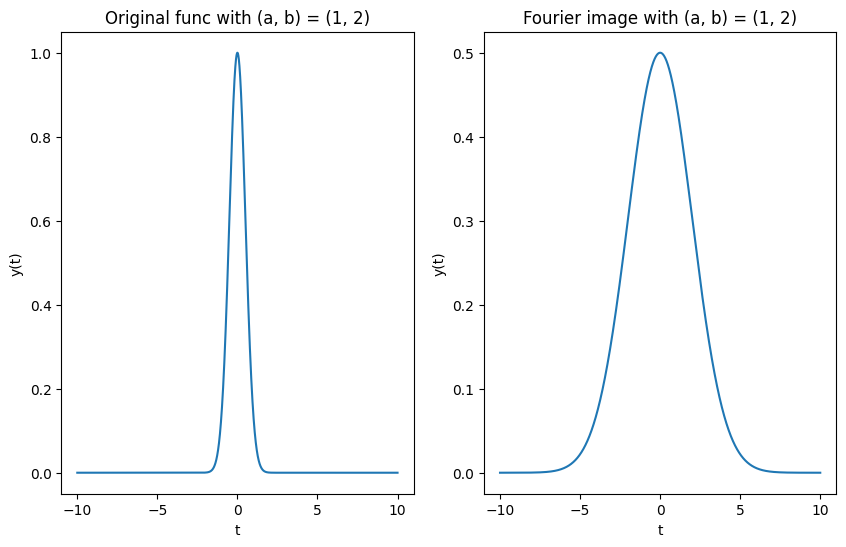
\includegraphics[width=0.9\textwidth]{f4_2.png}
    \caption{График и образ функции Гаусса}
\end{figure}

\begin{figure}[ht]
    \centering
    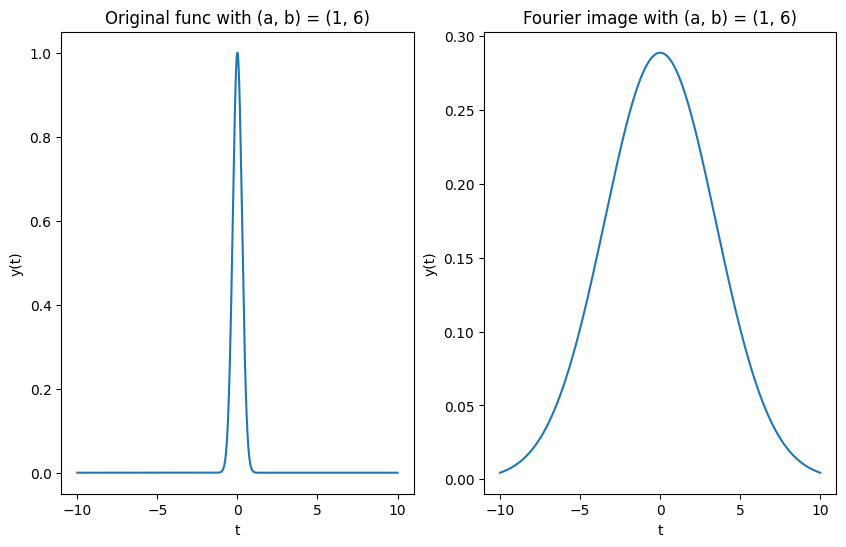
\includegraphics[width=0.9\textwidth]{f4_3.png}
    \caption{График и образ функции Гаусса}
\end{figure}

\newpage

\subsection{Равенство Парсеваля}

Получил \texttt{delta: 0.00000}, странно, что оба интеграла зануляются при любых $a,b$, поэтому их разность всегда нулевая\dots ещё предстоит разобраться.

\subsection{Анализ ситуации}

Влияние параметров $a$ и $b$ на функцию Гаусса можно понять по формулам образа и исходной функции.
Параметр $a$ отвечает за амплитуду функции, а параметр $b$ за ширину исходной функция.
то есть, при увеличении $a$ амплитуда функции увеличивается, при увеличении $b$ функция становится
уже, это можно заметить, исходя из графиков выше.

Также по графикам можно \textit{заметить}, что при некотором значении параматера $a$ и $b$ - функция и образ будут равны. Можно вывести эти параметры исходя из равентсва двух функций, 
а можно методом пристального взгляда на такое равенство увидеть, что сразу $a=1$, а потом  $b=1/2$ аккуратно причёсывает функции:

\begin{figure}[ht]
    \centering
    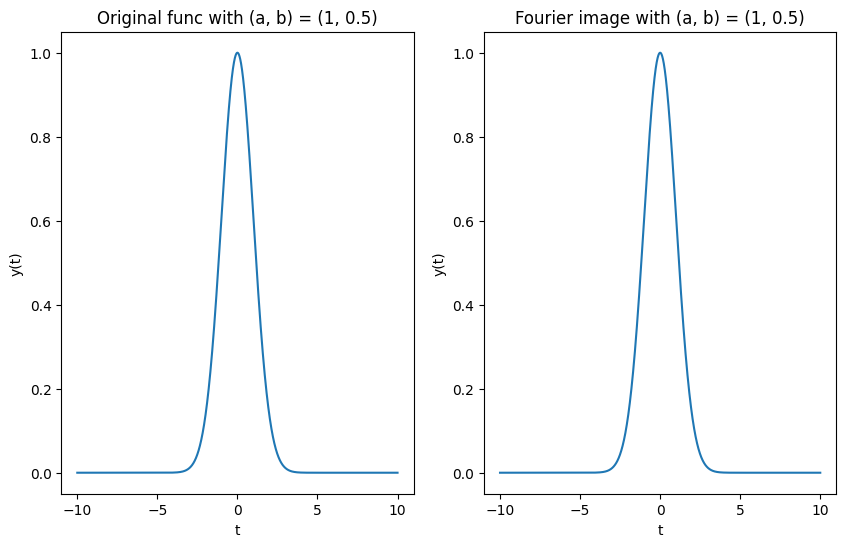
\includegraphics[width=0.9\textwidth]{f4_4.png}
    \caption{Равенство образа и функции функции Гаусса}
\end{figure}

\section{Двустороннее затухание}
$$
f(t) = ae^{-b|t|}
$$


\subsection{Фурье-Образ}

$\hat{f_5}(\omega) = \frac{1}{\sqrt{2\pi}}\int^{+\infty}_{-\infty}ae^{-b|t|}\cdot e^{-i\omega t} dt \\ =  \frac{a}{\sqrt{2\pi}}\bigg[\int^{0}_{-\infty}e^{bt}e^{-i\omega t} dt + \int^{+\infty}_{0}e^{-bt}e^{-i\omega t}dt  \bigg] = \\
\frac{a}{\sqrt{2\pi}}\bigg[\int^{0}_{-\infty}e^{t(b-i\omega)} dt + \int^{+\infty}_{0}e^{-t(b+i\omega)}dt  \bigg]=
\frac{a}{\sqrt{2\pi}} \big[ \frac{e^{t(b-i\omega)}}{b-i\omega}\bigr|_{-\infty}^0+ \frac{e^{-t(b+i\omega)}}{b+i\omega}\bigr|^{+\infty}_0 \big]= 
\frac{a}{\sqrt{2\pi}}  \big( \frac{1}{b-i\omega} + \frac{1}{b+i\omega} \big) = \frac{2ab}{\sqrt{2\pi}(\omega^2 + b^2)}$

\subsection{Графики функции и Фурье-образа}

\begin{figure}[ht]
    \centering
    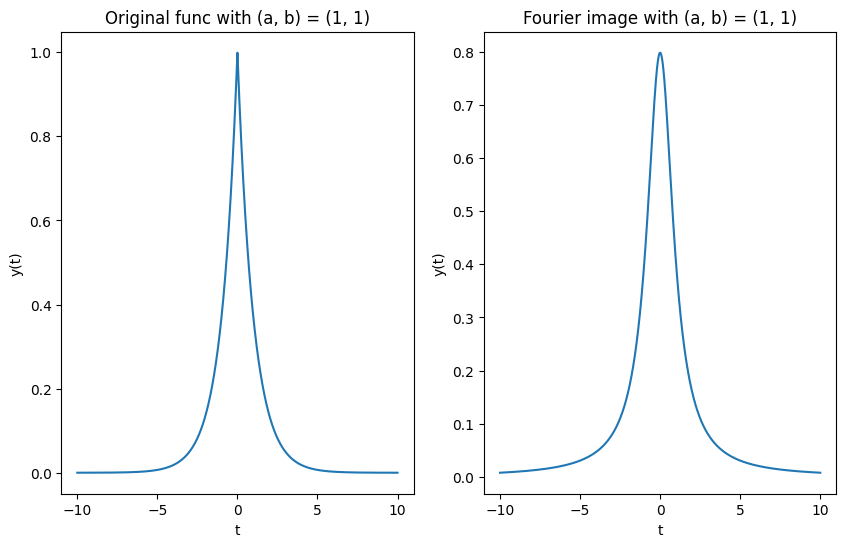
\includegraphics[width=0.9\textwidth]{f5_1.png}
    \caption{График и образ двустороннего затухания}
\end{figure}

\begin{figure}[ht]
    \centering
    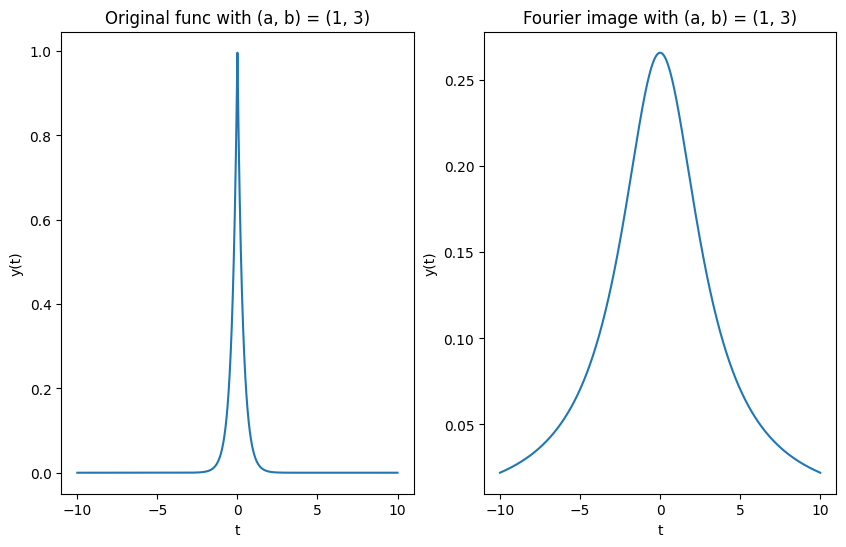
\includegraphics[width=0.9\textwidth]{f5_2.png}
    \caption{График и образ двустороннего затухания}
\end{figure}

\begin{figure}[ht]
    \centering
    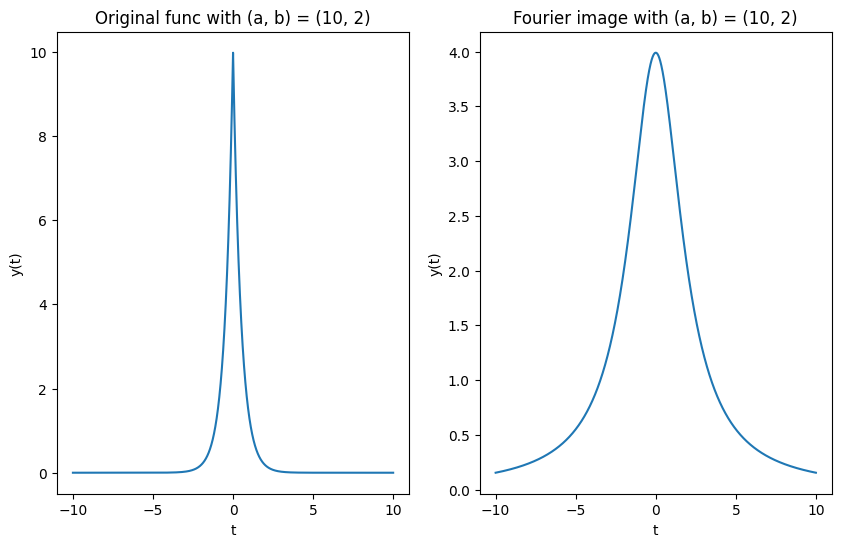
\includegraphics[width=0.9\textwidth]{f5_3.png}
    \caption{График и образ двустороннего затухания}
\end{figure}
\newpage

\subsection{Равенство Парсеваля}

Получил \texttt{delta: 0.00000}, а здесь уже только первый интеграл всегда равен нулю(надо разобраться), а второй - слишком малого порядка, поэтому их разность нулевая.


\subsection{Анализ ситуации}

Здесь влияние параметров $a$ и $b$ на графики функции возможно не заметно с первого взгляда, но если посмотреть на формулы исходной функции и образа, то всё станет понятнее:

$a$ отвечает за амплитуду функции, $b$ - за скорость затухания. При увеличении $a$ - амплитуда функции увеличивается, а при увеличении
$b$ функция затухает быстрее.

\endinput